results intro:
%   \arz{For this first paragraph, I might attempt to do something like the following. I think this
%   gives a nice introduction to the basic result, incorporates what the reader needs to know about
%   low-and high-mass stars (so we can remove that part from the introduction), and segues into
%   the separate subsections about low- and high-mass stars. This may need some editing, but I hope
%   you get the idea.}


hi mass Stars:
The contraction causes a temporary increase in $\Teff$ and a feature in the star's HR diagram called the convective hook (see Figures \ref{fig:tracks} and \ref{fig:isos_cb}).

% Teff plot
\begin{figure*}
  \centering
  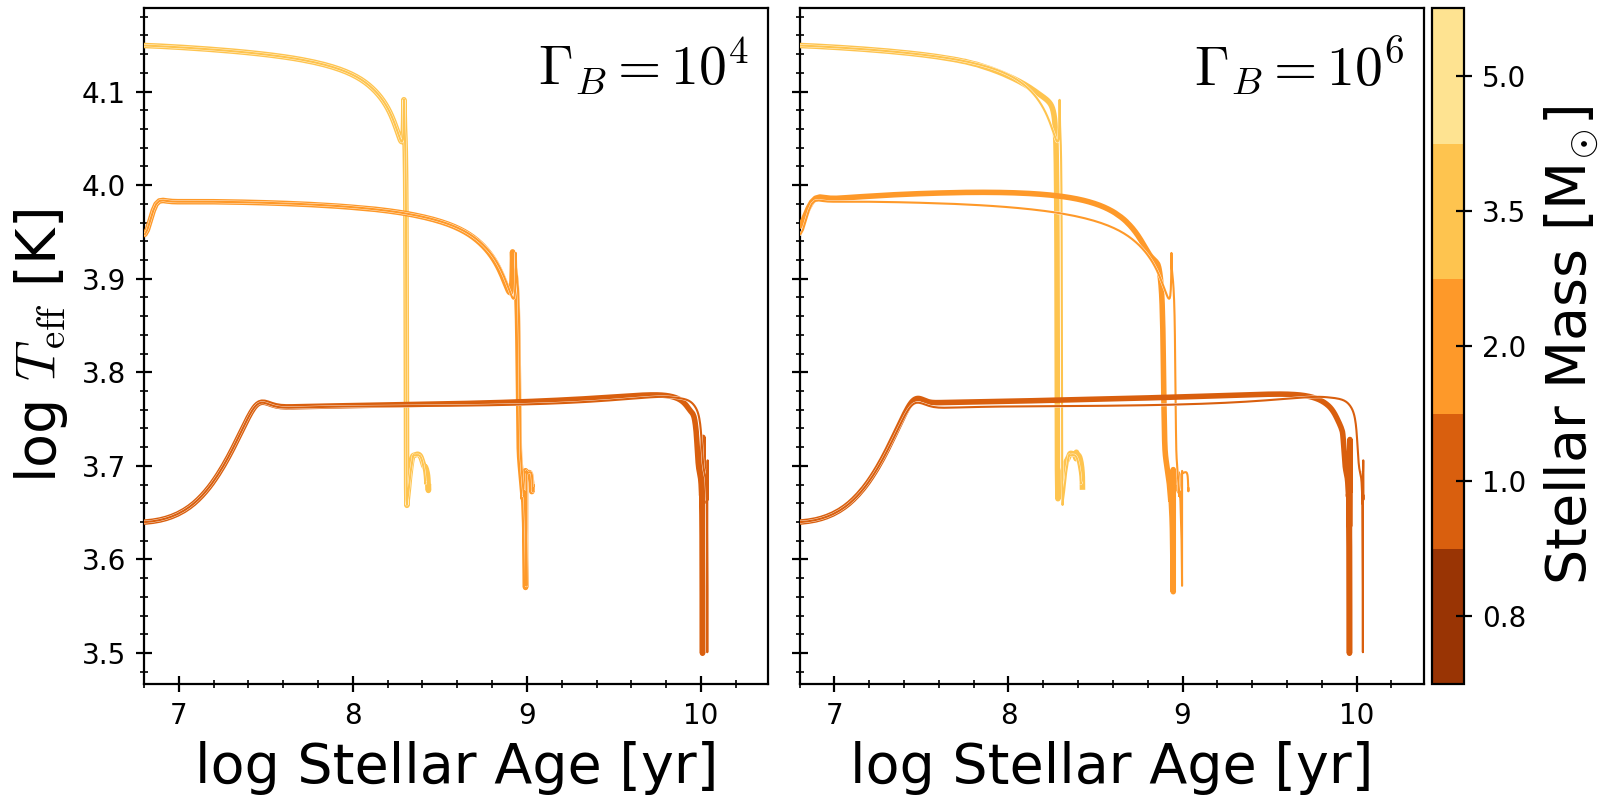
\includegraphics[width=\textwidth]{plots/Teff.png}
  \caption{$\Teff$ as a function of age for select $\gb$, with \nodm models overplotted as thin lines. Stars undergo a sharp decrease in $\Teff$ as they leave the MS. The change in MS lifetimes due to ADM can be seen in the time difference between these features. The surface effects of core oscillations discussed in \S~\ref{sub:lowmass} can be seen here in $\Teff$.
  }
  \label{fig:Teff}
\end{figure*}



% hottest MS Teff plots
\begin{figure*}
  \centering
  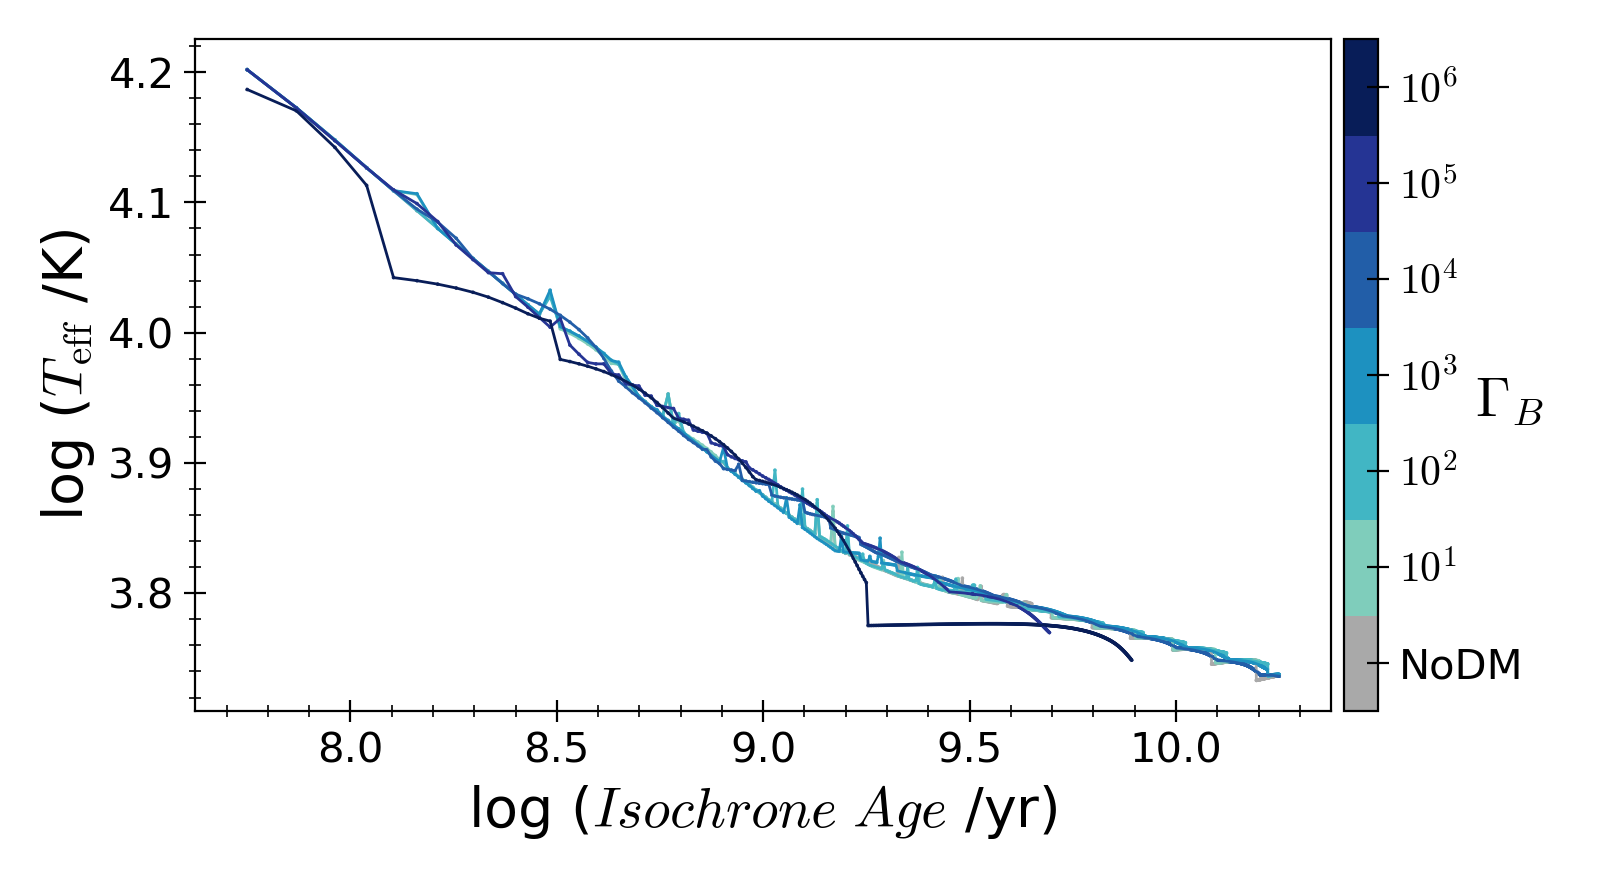
\includegraphics[width=\textwidth]{plots/hotTeff.png}
  \caption{
  Temperature of the hottest MS star. Models with $\gbpow{5}$ and $\gbpow{6}$ show significant decreases in $\Teff$ as higher mass stars leave the MS earlier than in \nodm models, leaving only cooler low mass stars.
  }
  \label{fig:hotTeff}

\end{figure*}




Notes:
hydrogen depletes in shell first. (low mass stars)
